% ==============================================================================
% SiteSync (সাইটসিংক) - Overleaf TikZ Diagrams
% Academic & Enterprise Architecture Specification Diagrams
% Instructions for Overleaf:
%   1. Create a new blank project on Overleaf (https://www.overleaf.com).
%   2. Replace the contents of main.tex with this file.
%   3. Set compiler to pdfLaTeX or XeLaTeX.
%   4. Click "Recompile" and download/screenshot the generated diagrams!
% ==============================================================================

\documentclass[11pt,a4paper]{article}
\usepackage[utf8]{inputenc}
\usepackage[margin=1in]{geometry}
\usepackage{tikz}
\usetikzlibrary{shapes.geometric, arrows.meta, positioning, calc, shadows, fit, backgrounds}
\usepackage{xcolor}
\usepackage{amsmath,amssymb}
\usepackage{caption}

% ---------------------------------------------------------
% Ukil Bhai Design System Palette Definitions
% ---------------------------------------------------------
\definecolor{primaryDark}{HTML}{223832}    % Deep Forest Slate
\definecolor{accentPeach}{HTML}{F5C29B}    % Soft Peach-Apricot
\definecolor{secondaryMuted}{HTML}{526B64} % Muted Forest Gray
\definecolor{tableTeal}{HTML}{2D4A43}      % Dark Teal
\definecolor{rowCream}{HTML}{F4F5F0}       % Warm Cream
\definecolor{alertRed}{HTML}{B9382C}       % Alert / Overbilling Red
\definecolor{fairGreen}{HTML}{10B981}      % Fair Market Green
\definecolor{discountBlue}{HTML}{2563EB}   % Discounted Bulk Blue
\definecolor{cardBg}{HTML}{FFFFFF}
\definecolor{borderDark}{HTML}{223832}

\tikzset{
    baseBox/.style = {
        rectangle,
        rounded corners=4pt,
        draw=borderDark,
        line width=1pt,
        minimum height=0.9cm,
        text centered,
        font=\small\sffamily,
        drop shadow={opacity=0.25, shadow xshift=1.5pt, shadow yshift=-1.5pt}
    },
    headerBox/.style = {
        baseBox,
        fill=tableTeal,
        text=white,
        font=\bfseries\small\sffamily,
        minimum height=1.0cm
    },
    accentBox/.style = {
        baseBox,
        fill=accentPeach,
        text=primaryDark,
        font=\bfseries\small\sffamily
    },
    standardBox/.style = {
        baseBox,
        fill=rowCream,
        text=primaryDark
    },
    alertBox/.style = {
        baseBox,
        fill=alertRed!15,
        draw=alertRed,
        text=alertRed,
        font=\bfseries\small\sffamily
    },
    greenBox/.style = {
        baseBox,
        fill=fairGreen!15,
        draw=fairGreen,
        text=fairGreen!80!black,
        font=\bfseries\small\sffamily
    },
    blueBox/.style = {
        baseBox,
        fill=discountBlue!15,
        draw=discountBlue,
        text=discountBlue,
        font=\bfseries\small\sffamily
    },
    pipelineArrow/.style = {
        ->,
        >={Stealth[length=6pt, width=5pt]},
        line width=1.4pt,
        color=tableTeal
    },
    subsystemGroup/.style = {
        draw=secondaryMuted,
        line width=1pt,
        dashed,
        rounded corners=6pt,
        inner sep=12pt,
        fill=black!2
    }
}

\begin{document}

\title{\textbf{\LARGE SiteSync (সাইটসিংক)}\\[0.3em]
\large System Architecture \& Multimodal Vision Pipeline Diagrams}
\author{\textbf{SiteSync Principal Engineering Group}}
\date{\today}
\maketitle

\vspace{1em}
\hrule
\vspace{1.5em}

% ==============================================================================
% DIAGRAM 1: 2-TIER OCR & LIVE MARKET PRICE INTELLIGENCE PIPELINE
% ==============================================================================
\section*{Figure 1: 2-Tier Challan OCR \& Market Intelligence Anti-Corruption Pipeline}

\begin{figure}[h!]
\centering
\begin{tikzpicture}[node distance=1.3cm and 1.8cm, auto]

    % Pipeline Nodes
    \node (camera) [accentBox, text width=3.2cm] {
        \textbf{CameraX Viewfinder}\\
        \footnotesize Tap-to-Focus, Auto-Torch,\\Bilingual Receipt Capture
    };

    \node (tier1) [standardBox, right=of camera, text width=3.4cm] {
        \textbf{Tier 1: On-Device ML Kit}\\
        \footnotesize Zero-Latency Text Boundary,\\Challan \#, Date \& Supplier
    };

    \node (tier2) [standardBox, right=of tier1, text width=3.8cm] {
        \textbf{Tier 2: Multimodal LLM}\\
        \footnotesize Gemini 1.5 Flash / Groq Vision\\
        Bilingual Line Items (বাংলা + Eng)
    };

    \node (brave) [headerBox, below=1.8cm of tier2, text width=3.8cm] {
        \textbf{Live Market Intelligence}\\
        \footnotesize Brave Search API Engine\\
        \textit{"\{material\} market price BD BDT"}
    };

    \node (variance) [standardBox, left=of brave, text width=3.4cm] {
        \textbf{Variance Algorithm}\\
        \footnotesize $\Delta = \frac{R_{\text{billed}} - R_{\text{bench}}}{R_{\text{bench}}} \times 100\%$
    };

    % Decision / Triage branches
    \node (triageFair) [greenBox, left=of variance, text width=3.2cm] {
        \textbf{FAIR\_MARKET}\\
        \footnotesize $|\Delta| \le 8\%$\\
        \checkmark Green Verified Check
    };

    \node (triageOver) [alertBox, above=0.6cm of triageFair, text width=3.2cm] {
        \textbf{OVER\_BILLED}\\
        \footnotesize $\Delta > +8\%$\\
        \textbf{!} Anti-Corruption Alert
    };

    \node (triageBulk) [blueBox, below=0.6cm of triageFair, text width=3.2cm] {
        \textbf{DISCOUNTED\_BULK}\\
        \footnotesize $\Delta < -8\%$\\
        $\star$ Bulk Savings Logged
    };

    \node (roomdb) [headerBox, below=1.8cm of variance, text width=8.5cm] {
        \textbf{Relational Room Database Engine (@Transaction)}\\
        \footnotesize Atomic Inventory Update: Stock IN Ledger $\cdot$ Material Recalculation $\cdot$ Cloud Sync
    };

    % Connectors
    \draw [pipelineArrow] (camera) -- node[above]{\footnotesize Image Uri} (tier1);
    \draw [pipelineArrow] (tier1) -- node[above]{\footnotesize Bounding Box} (tier2);
    \draw [pipelineArrow] (tier2) -- node[right]{\footnotesize Material List} (brave);
    \draw [pipelineArrow] (brave) -- node[above]{\footnotesize Benchmark Rate} (variance);
    
    \draw [pipelineArrow] (variance.west) -- ++(-0.6,0) |- (triageOver.east);
    \draw [pipelineArrow] (variance.west) -- (triageFair.east);
    \draw [pipelineArrow] (variance.west) -- ++(-0.6,0) |- (triageBulk.east);

    \draw [pipelineArrow] (variance.south) -- node[right]{\footnotesize Audited Bill Data} (roomdb.north);

\end{tikzpicture}
\caption{End-to-end 2-Tier OCR extraction, real-time Brave Search benchmarking, and automated tri-state anti-corruption triage.}
\end{figure}

\newpage

% ==============================================================================
% DIAGRAM 2: SITESYNC HIGH-LEVEL 3-TIER SYSTEM ARCHITECTURE
% ==============================================================================
\section*{Figure 2: SiteSync Clean MVVM 3-Tier Enterprise Architecture}

\begin{figure}[h!]
\centering
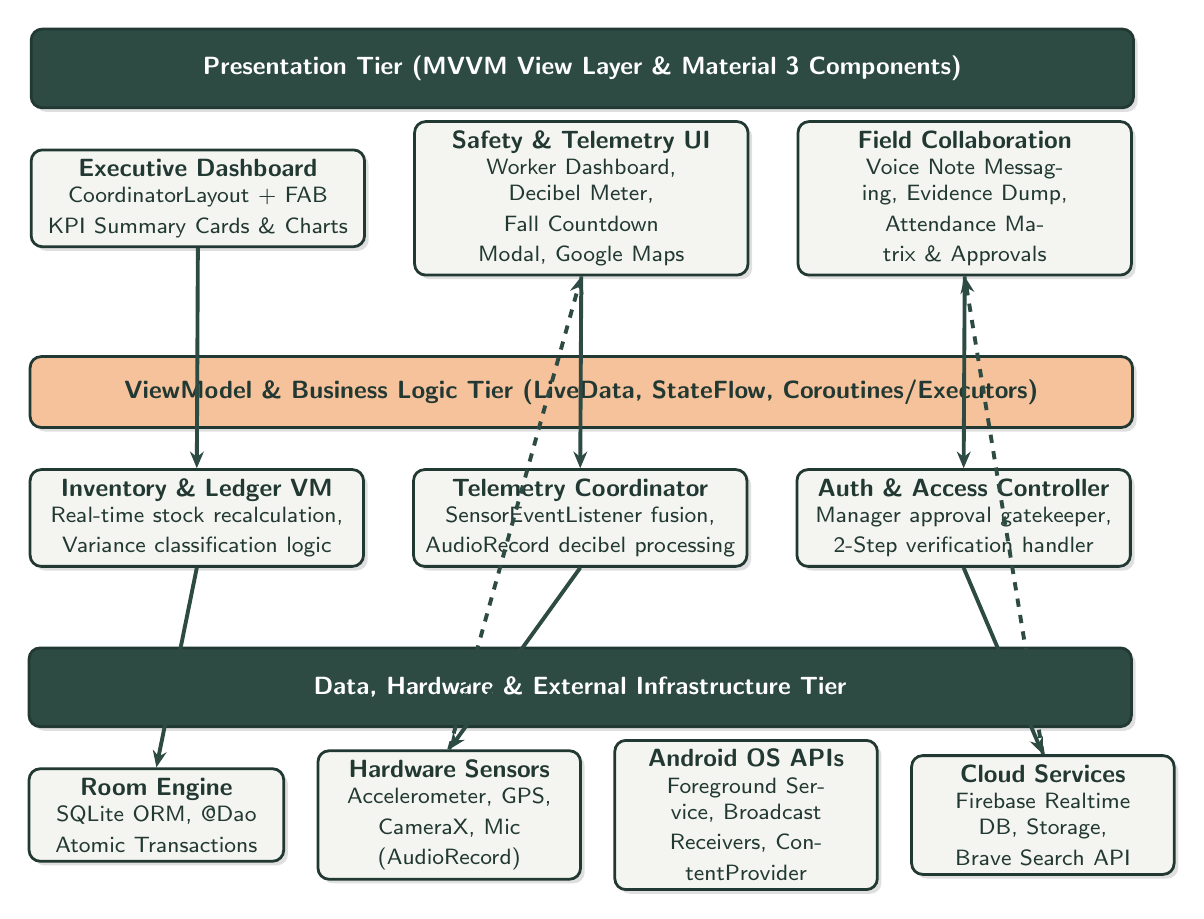
\begin{tikzpicture}[node distance=1.0cm and 1.2cm]

    % Presentation Tier
    \node (ui_header) [headerBox, minimum width=14cm] {\textbf{Presentation Tier (MVVM View Layer \& Material 3 Components)}};
    
    \node (dash_ui) [standardBox, below=0.5cm of ui_header.south west, anchor=north west, text width=4.0cm] {
        \textbf{Executive Dashboard}\\
        \footnotesize CoordinatorLayout + FAB\\
        KPI Summary Cards \& Charts
    };

    \node (safety_ui) [standardBox, right=0.6cm of dash_ui, text width=4.0cm] {
        \textbf{Safety \& Telemetry UI}\\
        \footnotesize Worker Dashboard, Decibel Meter,\\Fall Countdown Modal, Google Maps
    };

    \node (collab_ui) [standardBox, right=0.6cm of safety_ui, text width=4.0cm] {
        \textbf{Field Collaboration}\\
        \footnotesize Voice Note Messaging, Evidence Dump,\\Attendance Matrix \& Approvals
    };

    % Domain / ViewModel Tier
    \node (vm_header) [accentBox, below=1.0cm of safety_ui, minimum width=14cm] {
        \textbf{ViewModel \& Business Logic Tier (LiveData, StateFlow, Coroutines/Executors)}
    };

    \node (inv_vm) [standardBox, below=0.5cm of vm_header.south west, anchor=north west, text width=4.0cm] {
        \textbf{Inventory \& Ledger VM}\\
        \footnotesize Real-time stock recalculation,\\Variance classification logic
    };

    \node (telemetry_vm) [standardBox, right=0.6cm of inv_vm, text width=4.0cm] {
        \textbf{Telemetry Coordinator}\\
        \footnotesize SensorEventListener fusion,\\AudioRecord decibel processing
    };

    \node (auth_vm) [standardBox, right=0.6cm of telemetry_vm, text width=4.0cm] {
        \textbf{Auth \& Access Controller}\\
        \footnotesize Manager approval gatekeeper,\\2-Step verification handler
    };

    % Data & Hardware Integration Tier
    \node (data_header) [headerBox, below=1.0cm of telemetry_vm, minimum width=14cm] {
        \textbf{Data, Hardware \& External Infrastructure Tier}
    };

    \node (room_data) [standardBox, below=0.5cm of data_header.south west, anchor=north west, text width=3.0cm] {
        \textbf{Room Engine}\\
        \footnotesize SQLite ORM, @Dao\\
        Atomic Transactions
    };

    \node (hardware_data) [standardBox, right=0.4cm of room_data, text width=3.1cm] {
        \textbf{Hardware Sensors}\\
        \footnotesize Accelerometer, GPS,\\CameraX, Mic (AudioRecord)
    };

    \node (os_data) [standardBox, right=0.4cm of hardware_data, text width=3.1cm] {
        \textbf{Android OS APIs}\\
        \footnotesize Foreground Service, Broadcast\\Receivers, ContentProvider
    };

    \node (cloud_data) [standardBox, right=0.4cm of os_data, text width=3.1cm] {
        \textbf{Cloud Services}\\
        \footnotesize Firebase Realtime DB, Storage,\\Brave Search API
    };

    % Inter-tier connection arrows
    \draw [pipelineArrow] (dash_ui.south) -- (inv_vm.north);
    \draw [pipelineArrow] (safety_ui.south) -- (telemetry_vm.north);
    \draw [pipelineArrow] (collab_ui.south) -- (auth_vm.north);

    \draw [pipelineArrow] (inv_vm.south) -- (room_data.north);
    \draw [pipelineArrow] (telemetry_vm.south) -- (hardware_data.north);
    \draw [pipelineArrow] (auth_vm.south) -- (cloud_data.north);

    \draw [pipelineArrow, dashed] (hardware_data.north) -- (safety_ui.south);
    \draw [pipelineArrow, dashed] (cloud_data.north) -- (collab_ui.south);

\end{tikzpicture}
\caption{Three-tier architectural model delineating decoupled presentation, domain state management, and unified hardware/cloud persistence.}
\end{figure}

\newpage

% ==============================================================================
% DIAGRAM 3: RELATIONAL ROOM DATABASE SCHEMA (ER DIAGRAM)
% ==============================================================================
\section*{Figure 3: Relational Construction Database Entity-Relationship Schema}

\begin{figure}[h!]
\centering
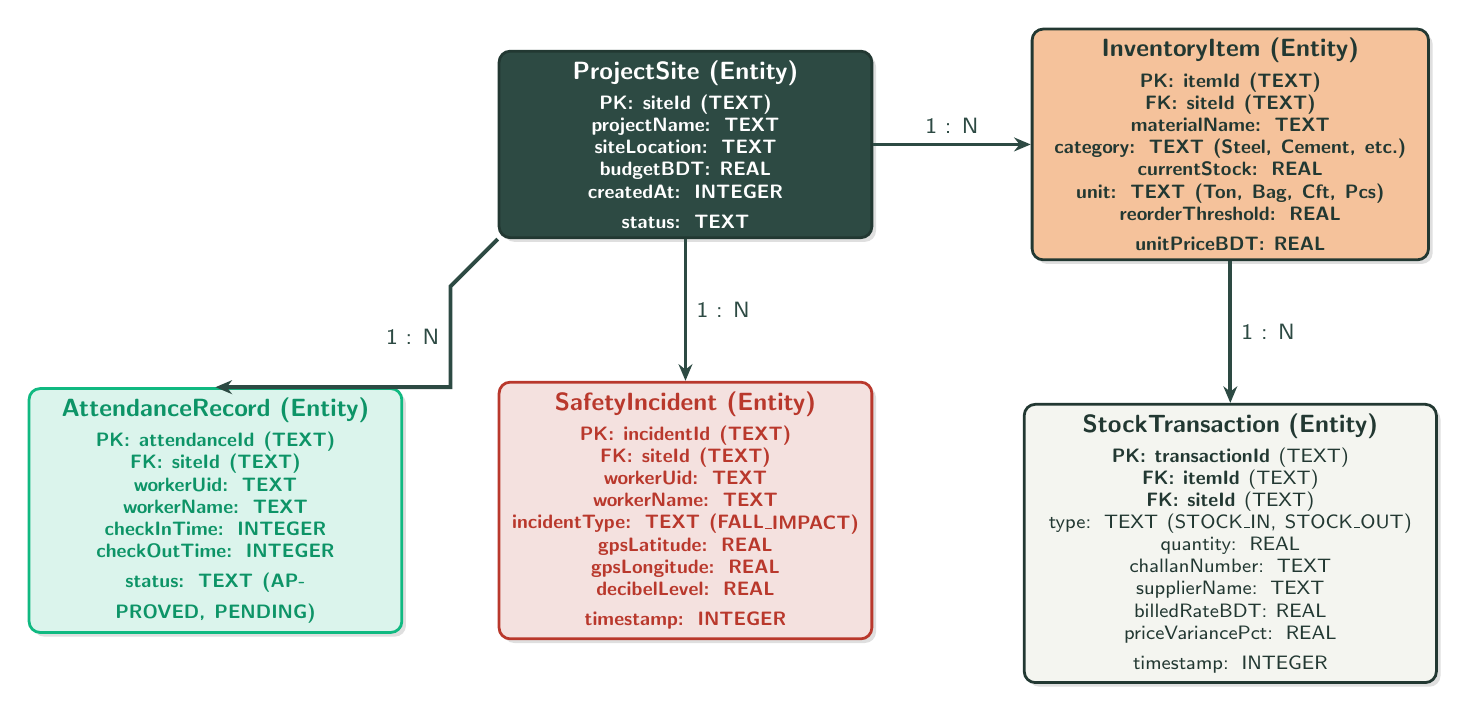
\begin{tikzpicture}[node distance=1.5cm and 2.0cm, every node/.style={font=\small\sffamily}]

    % Entity: Project Site
    \node (site) [headerBox, text width=4.5cm] {
        \textbf{ProjectSite (Entity)}\\[0.3em]
        \scriptsize
        \textbf{PK: siteId} (TEXT)\\
        projectName: TEXT\\
        siteLocation: TEXT\\
        budgetBDT: REAL\\
        createdAt: INTEGER\\
        status: TEXT
    };

    % Entity: Inventory Item
    \node (inventory) [accentBox, right=of site, text width=4.8cm] {
        \textbf{InventoryItem (Entity)}\\[0.3em]
        \scriptsize
        \textbf{PK: itemId} (TEXT)\\
        \textbf{FK: siteId} (TEXT)\\
        materialName: TEXT\\
        category: TEXT (Steel, Cement, etc.)\\
        currentStock: REAL\\
        unit: TEXT (Ton, Bag, Cft, Pcs)\\
        reorderThreshold: REAL\\
        unitPriceBDT: REAL
    };

    % Entity: Stock Transaction
    \node (transaction) [standardBox, below=1.8cm of inventory, text width=5.0cm] {
        \textbf{StockTransaction (Entity)}\\[0.3em]
        \scriptsize
        \textbf{PK: transactionId} (TEXT)\\
        \textbf{FK: itemId} (TEXT)\\
        \textbf{FK: siteId} (TEXT)\\
        type: TEXT (STOCK\_IN, STOCK\_OUT)\\
        quantity: REAL\\
        challanNumber: TEXT\\
        supplierName: TEXT\\
        billedRateBDT: REAL\\
        priceVariancePct: REAL\\
        timestamp: INTEGER
    };

    % Entity: Safety Incident
    \node (incident) [alertBox, below=1.8cm of site, text width=4.5cm] {
        \textbf{SafetyIncident (Entity)}\\[0.3em]
        \scriptsize
        \textbf{PK: incidentId} (TEXT)\\
        \textbf{FK: siteId} (TEXT)\\
        workerUid: TEXT\\
        workerName: TEXT\\
        incidentType: TEXT (FALL\_IMPACT)\\
        gpsLatitude: REAL\\
        gpsLongitude: REAL\\
        decibelLevel: REAL\\
        timestamp: INTEGER
    };

    % Entity: Attendance Record
    \node (attendance) [greenBox, left=1.2cm of incident, text width=4.5cm] {
        \textbf{AttendanceRecord (Entity)}\\[0.3em]
        \scriptsize
        \textbf{PK: attendanceId} (TEXT)\\
        \textbf{FK: siteId} (TEXT)\\
        workerUid: TEXT\\
        workerName: TEXT\\
        checkInTime: INTEGER\\
        checkOutTime: INTEGER\\
        status: TEXT (APPROVED, PENDING)
    };

    % Relations / Lines
    \draw [pipelineArrow] (site.east) -- node[above]{\footnotesize 1 : N} (inventory.west);
    \draw [pipelineArrow] (inventory.south) -- node[right]{\footnotesize 1 : N} (transaction.north);
    \draw [pipelineArrow] (site.south) -- node[right]{\footnotesize 1 : N} (incident.north);
    \draw [pipelineArrow] (site.south west) -- ++(-0.6,-0.6) |- node[near start, left]{\footnotesize 1 : N} (attendance.north);

\end{tikzpicture}
\caption{Room Database relational mapping featuring strict foreign keys, indexing, and atomic multi-site transaction tracing.}
\end{figure}

\newpage

% ==============================================================================
% DIAGRAM 4: SENSORY TELEMETRY & FALL EMERGENCY LIFECYCLE
% ==============================================================================
\section*{Figure 4: Sensory Telemetry \& Worker Fall Rescue State Machine}

\begin{figure}[h!]
\centering
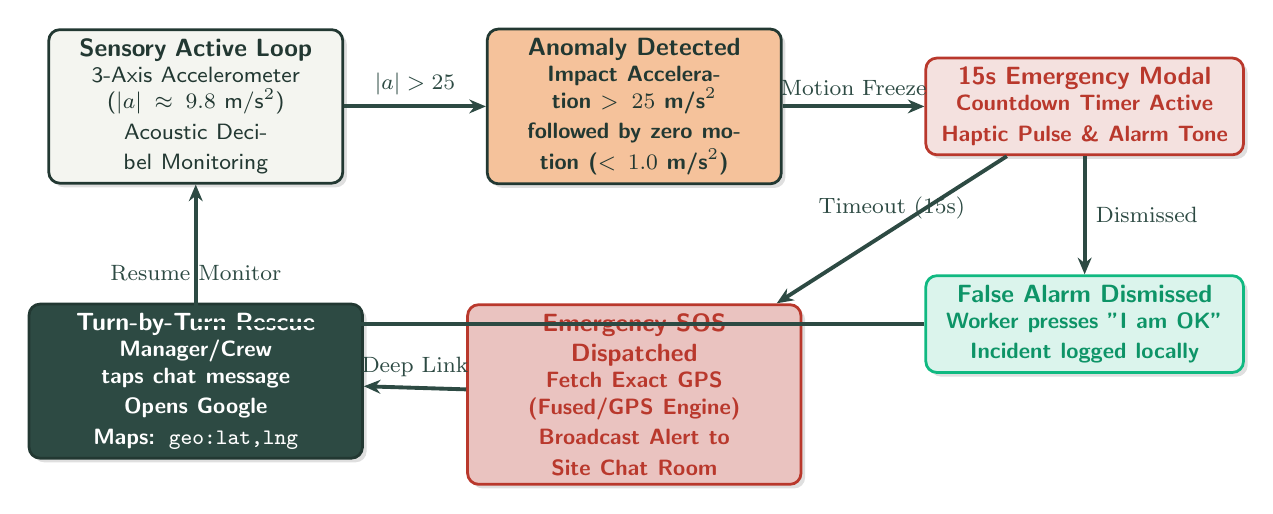
\begin{tikzpicture}[node distance=1.4cm and 1.8cm, auto]

    \node (monitoring) [standardBox, text width=3.5cm] {
        \textbf{Sensory Active Loop}\\
        \footnotesize 3-Axis Accelerometer ($|a| \approx 9.8\text{ m/s}^2$)\\
        Acoustic Decibel Monitoring
    };

    \node (anomaly) [accentBox, right=of monitoring, text width=3.5cm] {
        \textbf{Anomaly Detected}\\
        \footnotesize Impact Acceleration $> 25\text{ m/s}^2$\\
        followed by zero motion ($< 1.0\text{ m/s}^2$)
    };

    \node (countdown) [alertBox, right=of anomaly, text width=3.8cm] {
        \textbf{15s Emergency Modal}\\
        \footnotesize Countdown Timer Active\\
        Haptic Pulse \& Alarm Tone
    };

    \node (cancelled) [greenBox, below=1.5cm of countdown, text width=3.8cm] {
        \textbf{False Alarm Dismissed}\\
        \footnotesize Worker presses "I am OK"\\
        Incident logged locally
    };

    \node (sos) [alertBox, fill=alertRed!30, below=1.5cm of anomaly, text width=4.0cm] {
        \textbf{Emergency SOS Dispatched}\\
        \footnotesize Fetch Exact GPS (Fused/GPS Engine)\\
        Broadcast Alert to Site Chat Room
    };

    \node (rescue) [headerBox, below=1.5cm of monitoring, text width=4.0cm] {
        \textbf{Turn-by-Turn Rescue}\\
        \footnotesize Manager/Crew taps chat message\\
        Opens Google Maps: \texttt{geo:lat,lng}
    };

    % Transitions
    \draw [pipelineArrow] (monitoring) -- node[above]{\footnotesize $|a| > 25$} (anomaly);
    \draw [pipelineArrow] (anomaly) -- node[above]{\footnotesize Motion Freeze} (countdown);
    \draw [pipelineArrow] (countdown) -- node[right]{\footnotesize Dismissed} (cancelled);
    \draw [pipelineArrow] (countdown) -- node[above]{\footnotesize Timeout (15s)} (sos);
    \draw [pipelineArrow] (sos) -- node[above]{\footnotesize Deep Link} (rescue);
    \draw [pipelineArrow] (cancelled) -| node[below, near end]{\footnotesize Resume Monitor} (monitoring);

\end{tikzpicture}
\caption{Autonomous fall detection lifecycle with false-positive cancellation window and turn-by-turn emergency dispatch.}
\end{figure}

\end{document}
